\section{Регулятор на операционном усилителе}
Рассмотрим регулятор на рисунке \ref{fig:task5_reg}.
\begin{figure}[ht!]
    \centering
    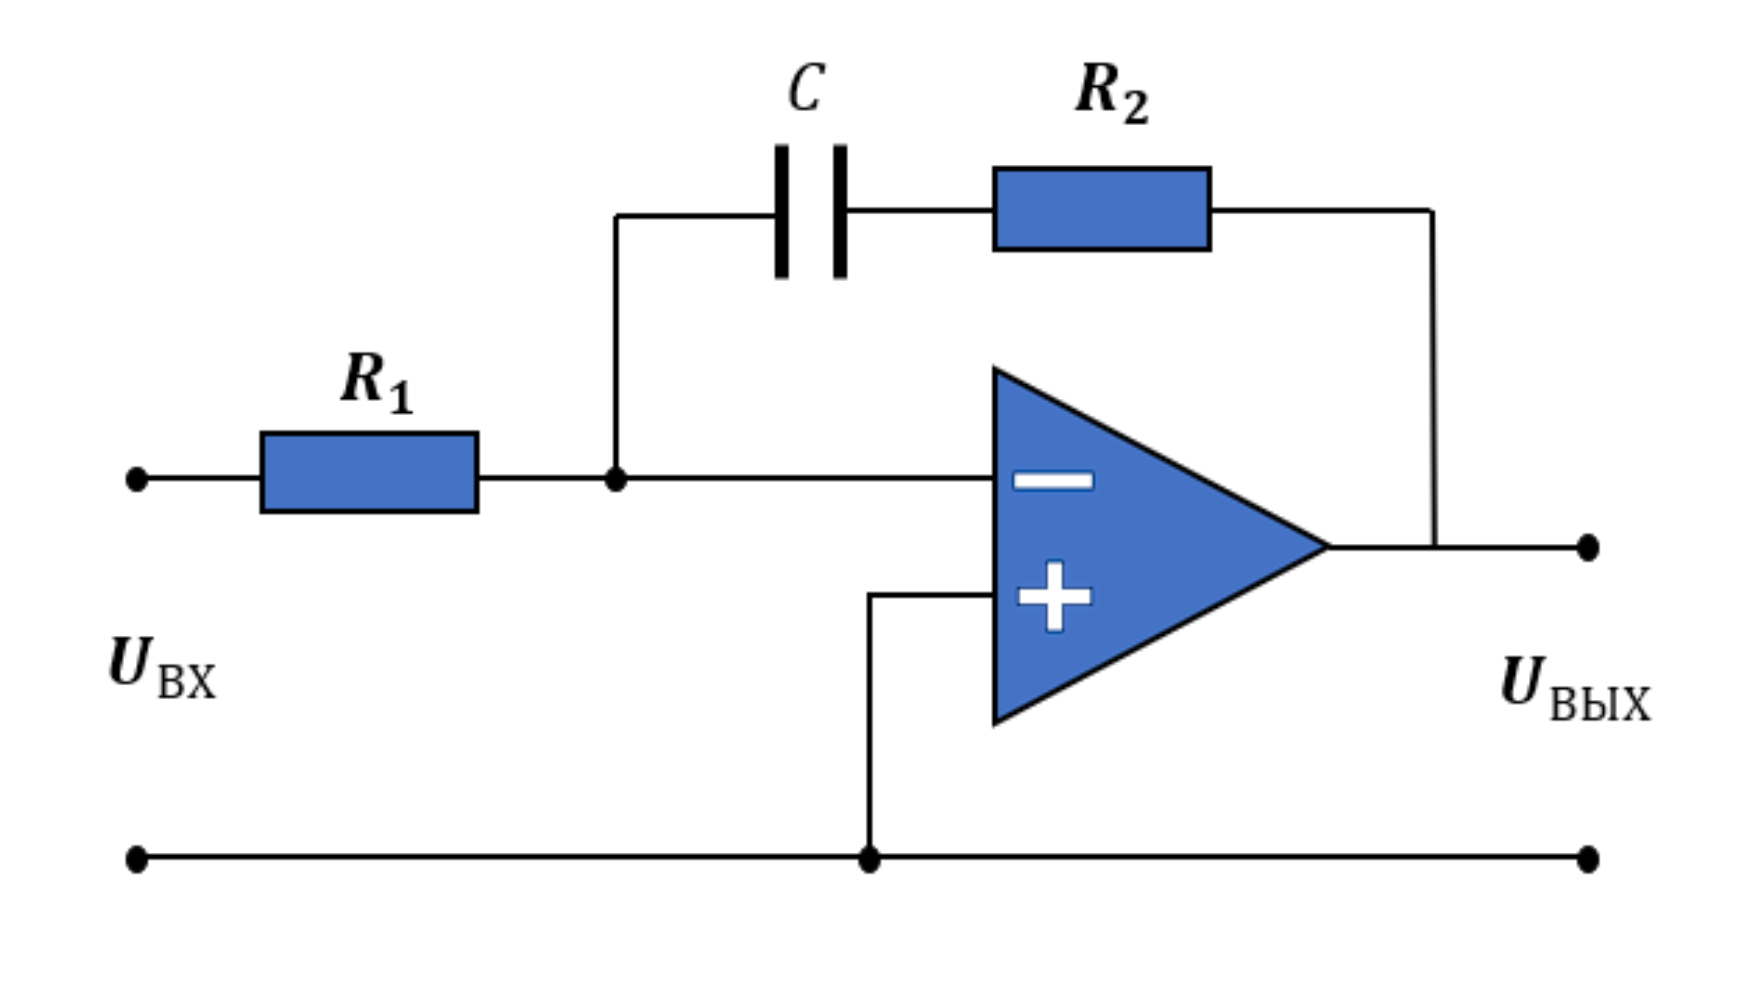
\includegraphics[width=0.8\textwidth]{media/reg.png}
    \caption{Регулятор на операционном усилителе}
    \label{fig:task5_reg}
\end{figure}
Его передаточная функция:
\begin{equation}
    W(s) = \frac{T_2s + 1}{T_1s}, \quad T_1 = R_1C, \quad T_2 = R_2C
\end{equation}

Данный регулятор соответствует стандартной структуре ПИ-регулятора, где $\frac{T_2}{T_1}$ -- пропорциональный коэффициент, а $\frac{1}{T_1}$ -- интегральный коэффициент.

\subsection{Временные характеристики}
\noindent Найдем весовую функцию системы:
\begin{equation}
    y_{\text{i.r.}}(t) = L^{-1}\left\{\frac{T_2s + 1}{T_1s}\right\} = \frac{T_2\delta(t) + 1}{T_1}
\end{equation}
Найдем переходную функцию:
\begin{equation}
    y_{\text{s.r.}}(t) = L^{-1}\left\{\frac{T_2s + 1}{T_1s}\cdot\frac{1}{s}\right\} = \frac{T_2 + t}{T_1}
\end{equation}

Сравнительные графики весовой и переходной функций, полученных аналитически и в ходе эксперимента  приведены на рис. \ref{fig:task5_impulse_response_cmp} и рис. \ref{fig:task5_step_response_cmp}.
\begin{figure}[ht!]
    \centering
    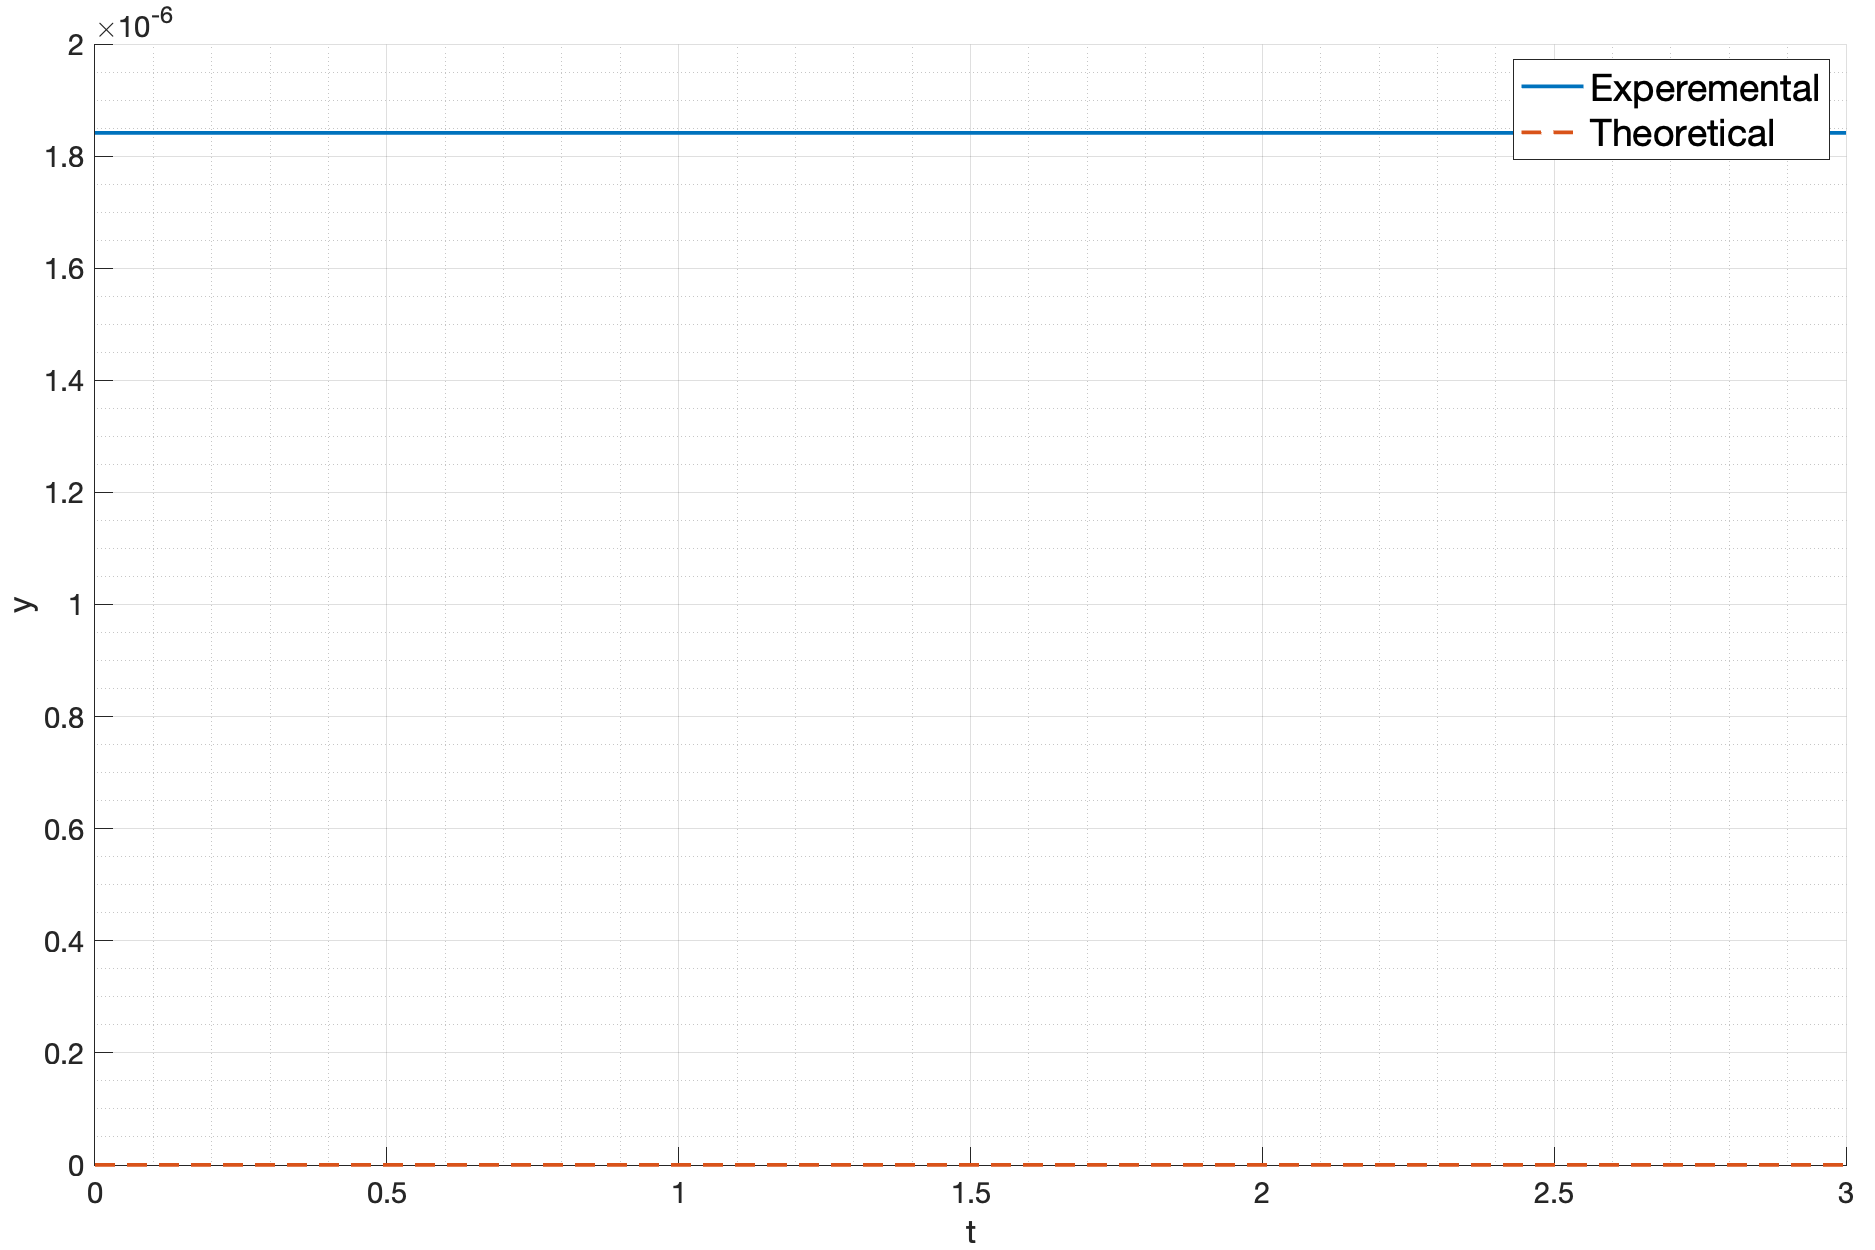
\includegraphics[width=\textwidth]{media/plots/task5_impulse_response_cmp.png}
    \caption{Сравнение весовых функций регулятора на операционном усилителе}
    \label{fig:task5_impulse_response_cmp}
\end{figure}
\begin{figure}[ht!]
    \centering
    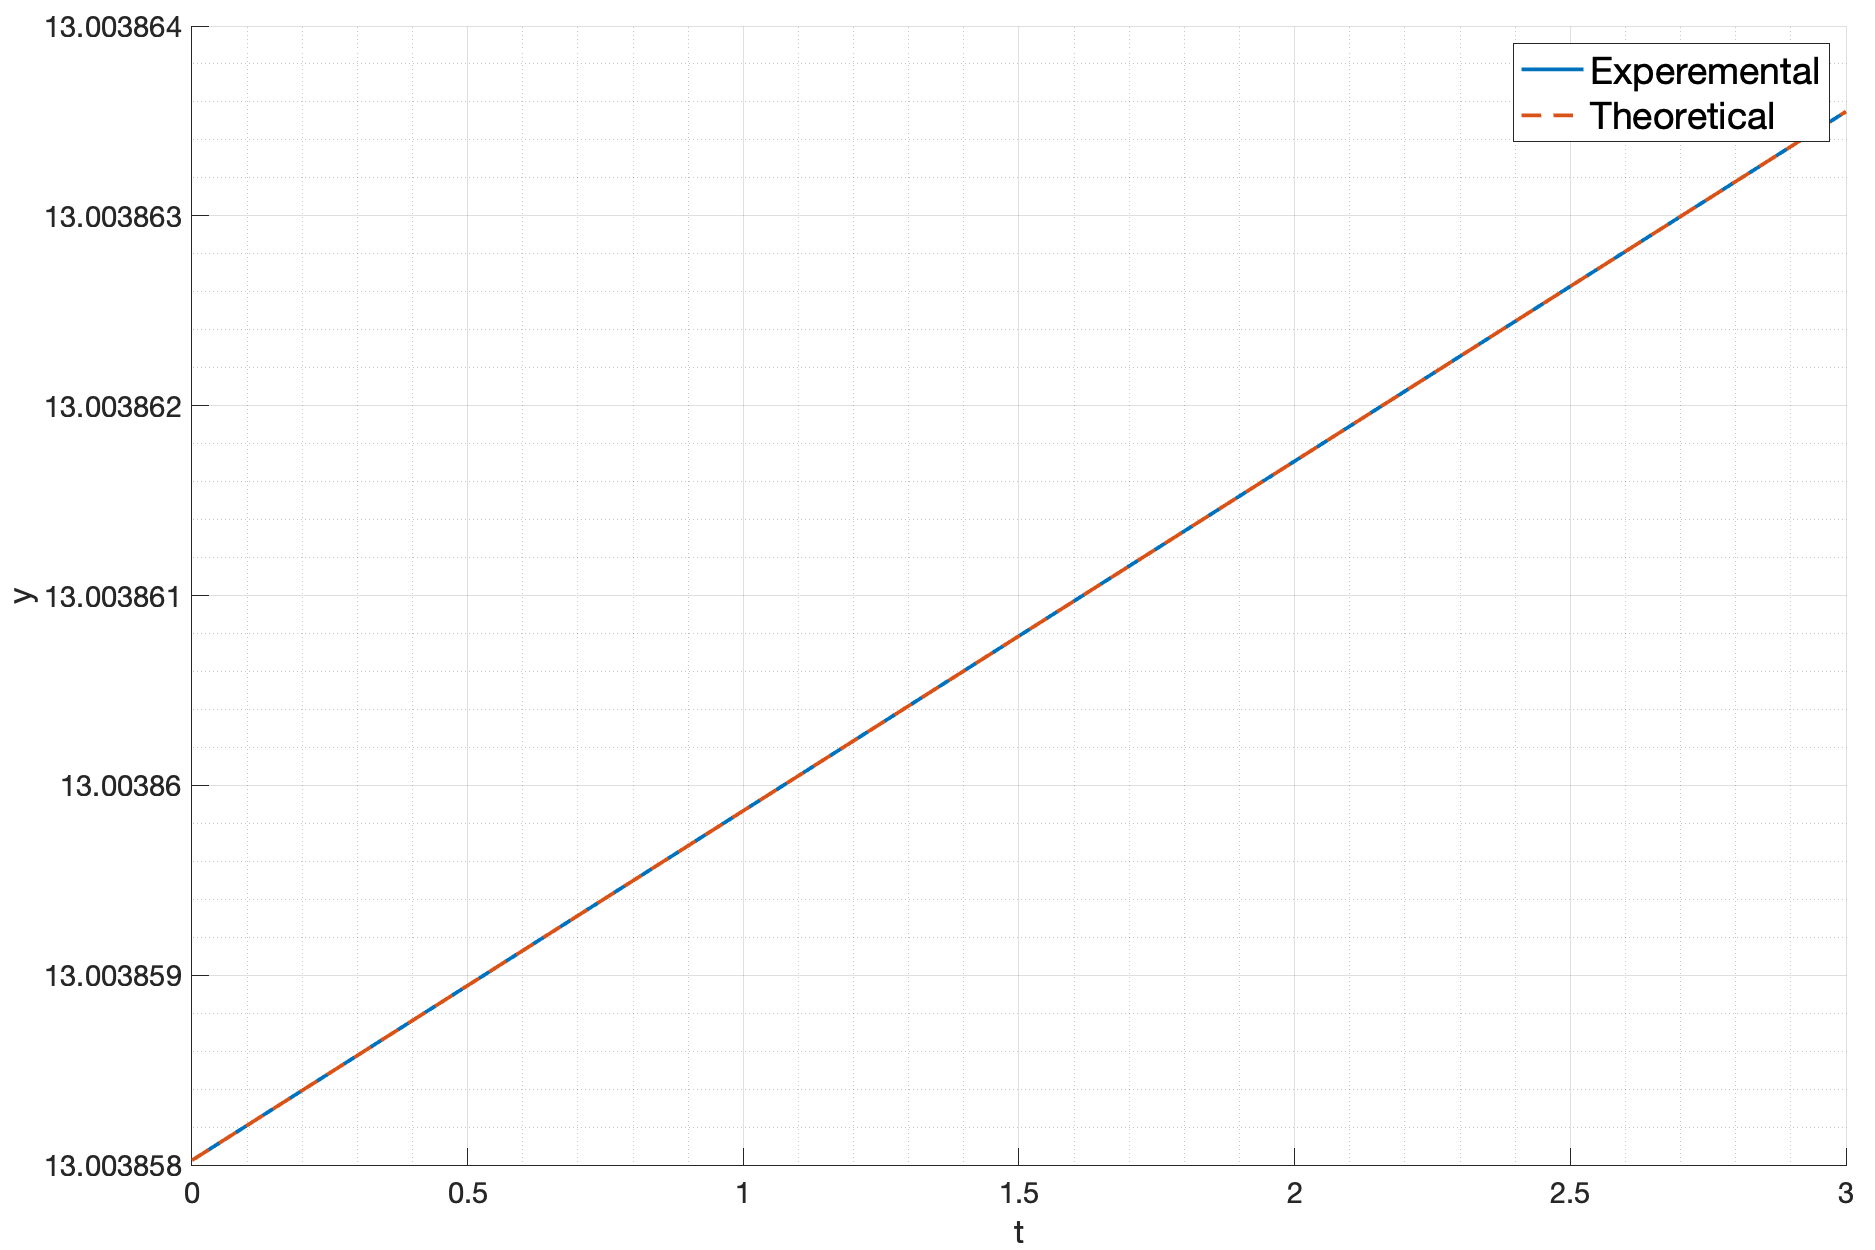
\includegraphics[width=\textwidth]{media/plots/task5_step_response_cmp.png}
    \caption{Сравнение переходных функций регулятора на операционном усилителе}
    \label{fig:task5_step_response_cmp}
\end{figure}

\FloatBarrier
\subsection{Частотные характеристики}
\noindent Найдем амплитудно-частотную характеристику и фазо-частотную характеристику,
\begin{equation}
    W(j\omega) = \frac{T_2j\omega + 1}{T_1j\omega} = \frac{T_2}{T_1} + \frac{j}{-T_1\omega}
\end{equation}
Амплитудная характеристика:
\begin{equation}
    A(\omega) = \sqrt{\left(\frac{T_2}{T_1}\right)^2 + \frac{1}{T_1^2\omega^2}}
\end{equation}
Фазовая характеристика:
\begin{equation}
    \varphi(\omega) = \text{atan2}\left(\frac{-1}{T_1\omega},~\frac{T_2}{T_1}\right)
\end{equation}

Сравнительные графики АЧХ, ФЧХ, ЛАЧХ, полученных аналитически и в ходе эксперимента, приведены на рис. \ref{fig:task5_freq_resp_cmp_lin} и рис. \ref{fig:task5_freq_resp_cmp_loglog}.
\begin{figure}[ht!]
    \centering
    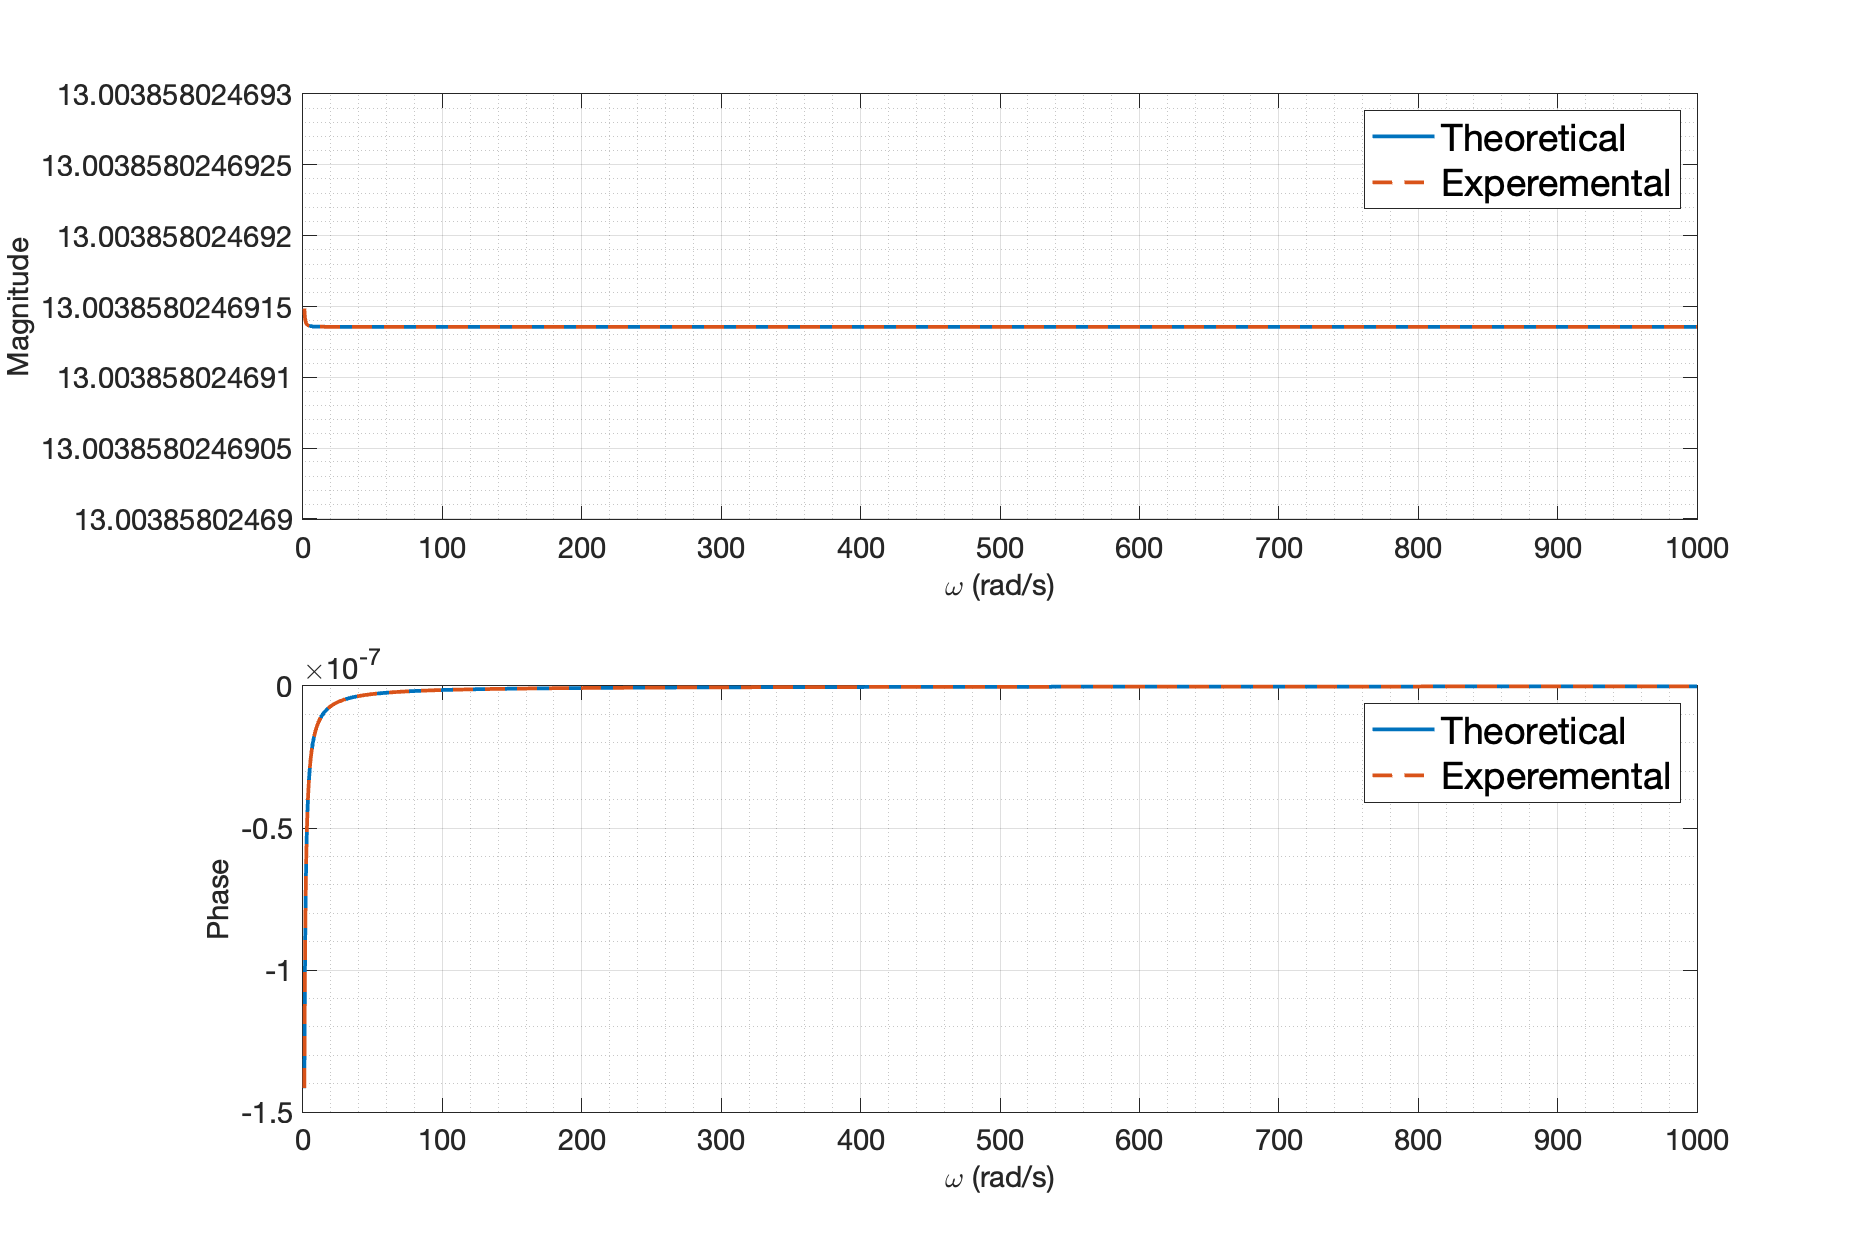
\includegraphics[width=\textwidth]{media/plots/task5_freq_resp_cmp_lin.png}
    \caption{Сравнение АЧХ и ФЧХ регулятора на операционном усилителе}
    \label{fig:task5_freq_resp_cmp_lin}
\end{figure}
\begin{figure}[ht!]
    \centering
    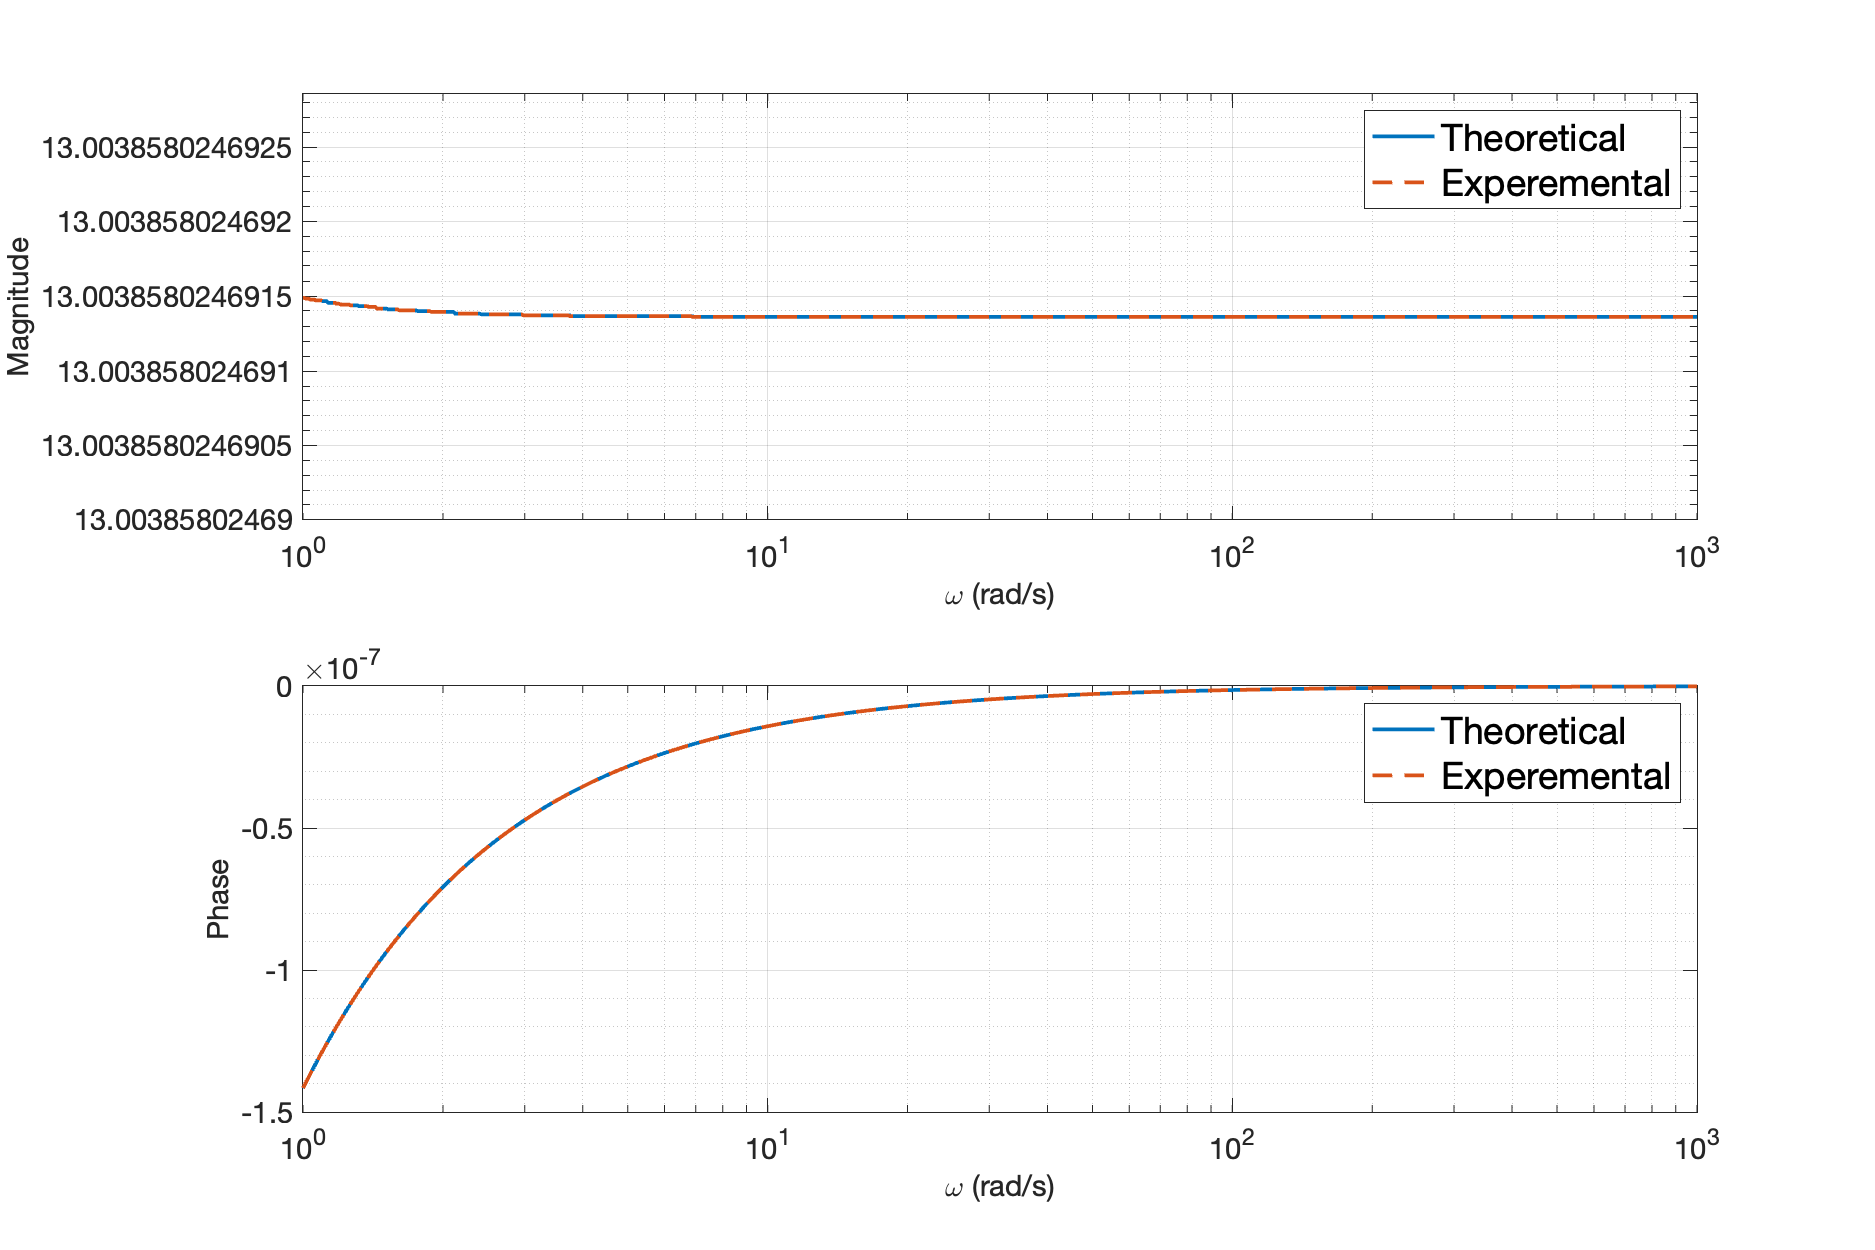
\includegraphics[width=\textwidth]{media/plots/task5_freq_resp_cmp_loglog.png}
    \caption{Сравнение логарифмической АЧХ регулятора на операционном усилителе}
    \label{fig:task5_freq_resp_cmp_loglog}
\end{figure}